\documentclass{report}
\usepackage[utf8]{inputenc}
\usepackage[a4paper, total={8in, 9in}]{geometry}
\usepackage{amsmath, amssymb}
\usepackage{bm}
\usepackage{graphicx}
\usepackage{subcaption}
\usepackage{caption}
\usepackage[colorlinks=true]{hyperref}

\title{Transition path sampling study of the MBHase reaction mechanism}
\author{Schwartz group}
\begin{document}
\maketitle

\section{Old variant}
\begin{figure}[ht!]
\begin{subfigure}{.5\textwidth}
  \centering
  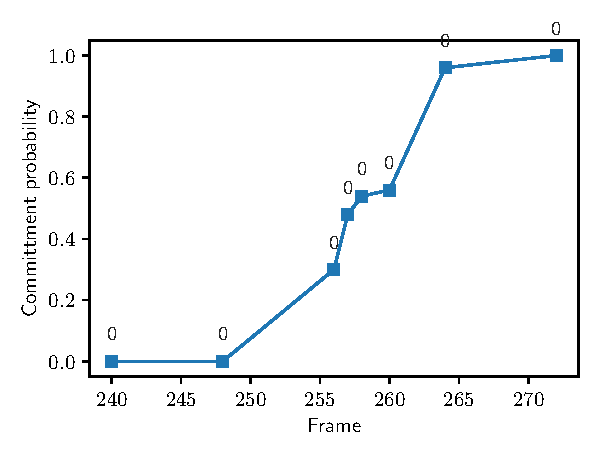
\includegraphics[width=.8\linewidth]{figures/dist72.pdf}
  %\caption{window 1}
  \label{fig:sfig1}
\end{subfigure}%
\begin{subfigure}{.5\textwidth}
  \centering
  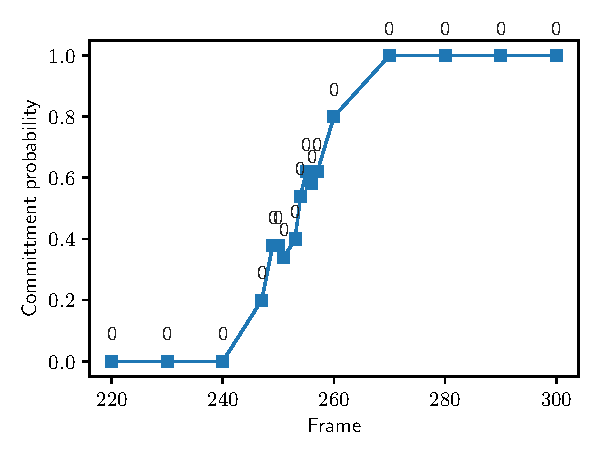
\includegraphics[width=.8\linewidth]{figures/dist100.pdf}
  %\caption{window 2}
  \label{fig:sfig2}
\end{subfigure}
\label{fig:fig}
\end{figure}

%\begin{figure}
%\begin{subfigure}{.5\textwidth}
%  \centering
%  \includegraphics[width=.8\linewidth]{figures/200_t.png}
  %\caption{window 5}
%  \label{fig:sfig1}
%\end{subfigure}%
%\begin{subfigure}{.5\textwidth}
%  \centering
%  \includegraphics[width=.8\linewidth]{figures/400_t.png}
  %\caption{window 6}
%  \label{fig:sfig2}
%\end{subfigure}
%\label{fig:fig}
%\end{figure}

%\begin{figure}
%\begin{subfigure}{.5\textwidth}
%  \centering
%  \includegraphics[width=0.9\textwidth]{figures/den-fenergy.pdf}
  %\caption{Unshifted free energies calculated for individual windows}
%  \label{fig:sfig1}
%\end{subfigure}%
%\begin{subfigure}{.5\textwidth}
%  \centering
%  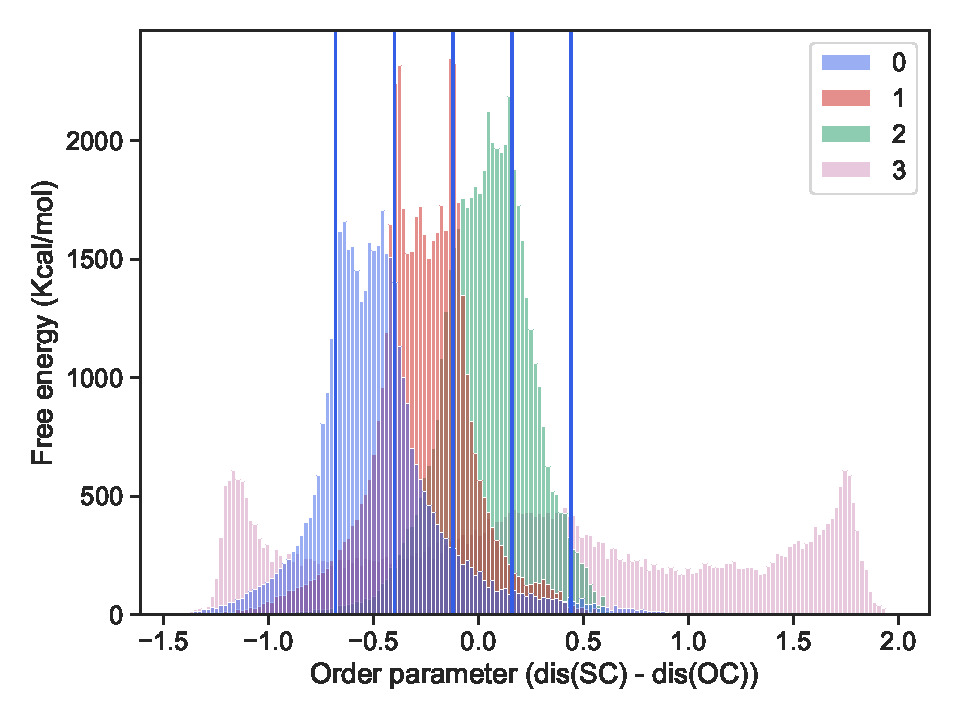
\includegraphics[width=0.9\textwidth]{figures/dist.pdf}
  %\caption{Free energies shifted in individual windows to match the values in overlapping regions}
%  \label{fig:sfig2}
%\end{subfigure}
%\caption{plots of....}
%\label{fig:fig}
%\end{figure}

\end{document}
